\documentclass[11pt]{article}
\usepackage[utf8]{inputenc}
\usepackage[T1]{fontenc}
\usepackage[margin=1in]{geometry}
\usepackage{amsmath,amssymb}
\usepackage{natbib}
\usepackage{graphicx}
\graphicspath{{figures/}}
\usepackage{booktabs}
\usepackage{caption}
\usepackage[hidelinks]{hyperref}
\captionsetup{font=small,labelfont=bf}
\setlength{\parskip}{2pt}
\setlength{\emergencystretch}{3em}

\title{\bfseries Anisotropic spacing of drumlins: transverse quasi-regularity at the
bedform scale versus along-flow clustering in the BRITICE record}
\author{R.~Chen\\{\small GUT Geoservice Inc., Montr\'eal, Qu\'ebec, Canada}}
\date{\today}

\begin{document}
\maketitle

\begin{abstract}
\noindent
Drumlins are widely interpreted as the emergent product of a subglacial bed-flow instability that
selects a characteristic wavelength, and large-sample studies report that drumlin fields are
statistically ``patterned'' rather than random. Because drumlins are strongly elongate, however, the
sense in which they are regularly spaced has not been resolved. We analyse 41\,702 drumlin outlines
from the BRITICE v2 compilation of Great Britain, reduce each to a centroid with a flow-parallel
long-axis azimuth and a width, segment the data into coherent single-flow fields, and decompose the
spacing into directions parallel and transverse to ice flow. Isotropic nearest-neighbour statistics
are \emph{clustered}, not regular (Clark--Evans $R\le1$ in all nine fields analysed, median $0.89$):
at the centroid level drumlins form along-flow trains. The regularity is purely \emph{transverse}: in
flow-aligned coordinates the across-flow pair correlation shows hard-core exclusion and a characteristic
spacing $\lambda_\perp\!\approx\!250$\,m, of the same order as the drumlin width ($\sim$250\,m). Compared
with a width-matched hard-rod (Tonks-gas) null, the transverse first-neighbour spacing is largely accounted
for by steric exclusion, with only weak longer-range transverse periodicity beyond it. The structure
factor is dominated by field patchiness at low wavenumber and is featureless at the spacing scale, so the
pattern is not hyperuniform. Drumlin ``spacing regularity'' is therefore an anisotropic, transverse,
bedform-width-scale phenomenon rather than an isotropic lattice-like or hyperuniform order --- a
distinction that constrains how spacing statistics should be used to test bed-instability theories.
\end{abstract}

\section{Introduction}
Drumlins --- streamlined hills of sediment formed beneath ice sheets and aligned with ice flow --- are
the most abundant subglacial bedform, yet their formation remains debated. A leading family of
hypotheses holds that drumlins are an emergent instability of the coupled flow of ice and deforming
till: a flat bed is unstable, and the fastest-growing mode selects a characteristic wavelength, so that
bedforms should be quasi-regularly spaced \citep{hindmarsh1998,fowler2000,fowler2014}. Because the
instability wavelength is predicted to set the bedform size as well as its spacing, regular spacing and a
preferred size are expected to appear together.

Empirically, \citet{clark2018spatial} examined 42\,000 drumlins from Britain, Ireland, Canada and Norway
with inhomogeneous spatial statistics and concluded that ``patterning is a near-ubiquitous property of
drumlins,'' with a regularity signal across length scales of roughly 100--1200\,m. That study treated the
spacing as an isotropic property. Drumlins are, however, strongly elongate (typical length-to-width
ratios of 2--4), so a single ``spacing'' conflates two very different geometries: the along-flow
arrangement of bedforms in trains and the across-flow arrangement of neighbouring trains. The instability
wavelength of the theory is intrinsically \emph{transverse} (incipient ridges grow across flow and are
later dissected into individual drumlins), so a physically meaningful test of regular spacing must
separate the two directions. It is also unknown whether any transverse spacing is independent of the
bedform width, or simply reflects the fact that drumlins, being finite-width objects, cannot overlap
side by side.

Here we use the BRITICE v2 drumlin compilation \citep{clark2018britice} to decompose drumlin spacing
into along-flow and transverse components, to test whether any transverse regularity exceeds simple
steric (non-overlap) packing at the drumlin width, and to ask whether the pattern is hyperuniform ---
i.e.\ whether long-wavelength density fluctuations are suppressed \citep{torquato2018}. The analysis uses
only open data and standard, edge-corrected point-pattern and structure-factor statistics.

\section{Data}
The BRITICE v2 GIS database \citep{clark2018britice} compiles glacial landforms of the last
British--Irish Ice Sheet from more than 1800 sources, in the British National Grid (metres). We use the
filtered \textit{Subglacial lineations (polygons)} layer, whose attribute table classifies 41\,702
features as drumlins (the more elongate mega-scale glacial lineations are mapped as crest-lines in a
separate layer and are not used here). Each drumlin polygon is reduced to its area-weighted centroid; a
principal-axis decomposition of the outline gives the long-axis azimuth (taken as the local ice-flow
direction) and the width (minor-axis extent). Across the dataset the median width is $\sim$250\,m and the
median length $\sim$750\,m, consistent with published drumlin dimensions.

\section{Methods}
\paragraph{Field segmentation.}
Drumlins occur in discrete fields separated by drumlin-free ground, and flow direction varies between
fields; pooling them would superpose distinct processes. We link drumlins whose centroids lie within
three median nearest-neighbour distances and take the connected components as fields. Inference is
restricted to coherent fields with at least 300 drumlins and a high azimuth concentration (axial mean
resultant length $\bar R_\theta\ge0.72$), giving nine fields of 504--1547 drumlins.

\paragraph{Isotropic and directional pair statistics.}
For each field we compute the Clark--Evans nearest-neighbour index $R$ \citep{clark1954} against a
Monte-Carlo complete-spatial-randomness (CSR) null in the matched convex hull ($R>1$ dispersed, $R<1$
clustered). We then rotate the field into flow-aligned coordinates (long-axis azimuth along the
$y$-axis) and compute directional pair correlations: the along-flow $g_\parallel$ and the transverse
$g_\perp$, each accumulated from pairs lying within a thin slab (0.5\,km) of the perpendicular
coordinate so that the one-dimensional spacing in each direction is isolated. The isotropic $g(r)$ is
also computed for reference.

\paragraph{Steric (hard-rod) null.}
To test whether transverse regularity exceeds simple non-overlap packing, we compare $g_\perp$ to an
equilibrium one-dimensional hard-rod (Tonks-gas) null in which each slab is repopulated with the same
number of rods of diameter equal to the measured drumlin width, placed at random subject to
non-overlap. The envelope of this null is the spacing expected from steric exclusion alone at the
observed density and width.

\paragraph{Structure factor.}
The radially averaged structure factor $S(k)=N^{-1}\big|\sum_j e^{-i\mathbf k\cdot\mathbf r_j}\big|^2$,
evaluated at the wavevectors of the bounding window, tests for hyperuniformity: a vanishing
$S(k\!\to\!0)$ would indicate suppressed long-wavelength density fluctuations \citep{torquato2018},
whereas a packing peak with finite $S(k\!\to\!0)$ indicates a liquid-like spacing.

\section{Results}

\subsection{Isotropic statistics: clustering, not regularity}
At the centroid level the drumlin fields are \emph{clustered}. The Clark--Evans index is $\le1$ in all
nine fields (median $R=0.89$; Fig.~\ref{fig:summary}b), and the isotropic $g(r)$ rises to $2$--$3$ at
small separations and decays monotonically (Fig.~\ref{fig:rep}, centre) --- the signature of
clustering, with no hard-core and no packing peak. The along-flow pair correlation $g_\parallel$ is also
$>1$ at short range (Fig.~\ref{fig:rep}, centre): drumlins are arranged in along-flow trains. Thus the
naive expectation of isotropic regular spacing is not met; isotropic nearest-neighbour regularity is
absent.

\begin{figure}[t]
\centering

\includegraphics[width=0.5\textwidth]{drumlin_map.pdf}
\caption{BRITICE v2 drumlins of Great Britain (41\,702 centroids), coloured by long-axis (ice-flow)
azimuth. Drumlins occur in discrete fields, each with a locally coherent flow direction; field
boundaries coincide with abrupt azimuth changes.}
\label{fig:map}
\end{figure}

\subsection{Transverse quasi-regularity at the bedform scale}
The regularity is entirely transverse. In flow-aligned coordinates the across-flow pair correlation
$g_\perp$ shows clear hard-core exclusion at small separation and a characteristic-spacing peak
(Fig.~\ref{fig:rep}, right). The transverse spacing is $\lambda_\perp\!\approx\!250$\,m (median over the
nine fields), of the same order as the median drumlin width ($\sim$250\,m); across fields
$\lambda_\perp$ tracks the drumlin width to within a factor of about two (Fig.~\ref{fig:summary}a). The
pattern is therefore strongly anisotropic: clustered along flow, quasi-regular across flow, at a
transverse scale set by the bedform width.

\begin{figure}[t]
\centering
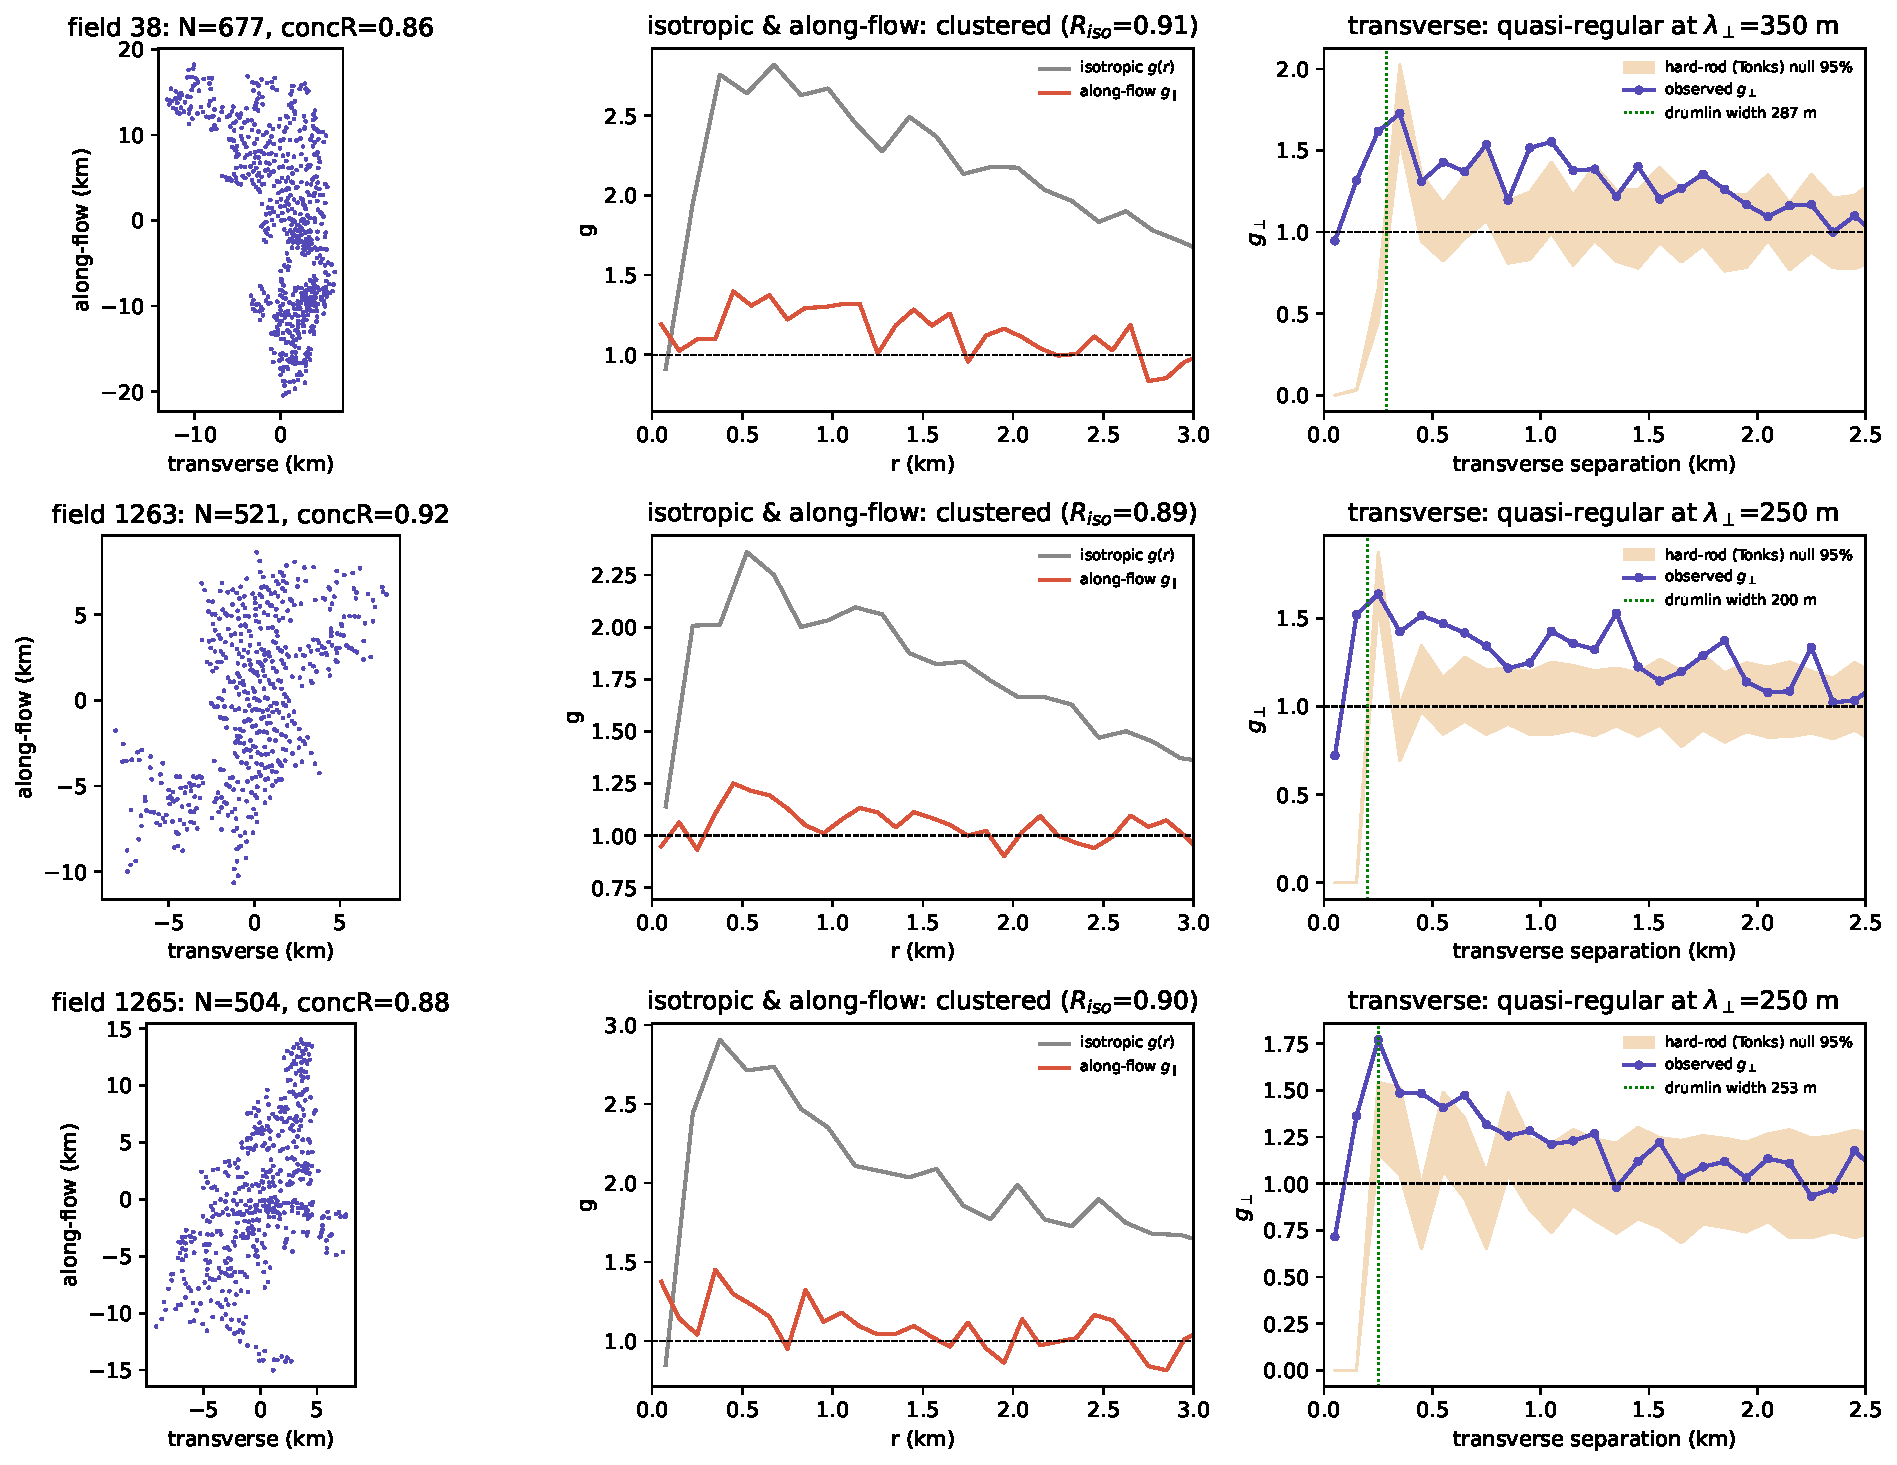
\includegraphics[width=\textwidth]{drumlin_rep.pdf}
\caption{Three representative coherent drumlin fields. Left: centroids in flow-aligned coordinates.
Centre: the isotropic $g(r)$ (grey) and along-flow $g_\parallel$ (red) are both $>1$ at short range
(clustering; $R_{\mathrm{iso}}<1$). Right: the transverse $g_\perp$ (purple) shows hard-core exclusion
and a characteristic spacing $\lambda_\perp$ near the drumlin width (green line); the shaded band is the
95\% envelope of a width-matched hard-rod (steric) null.}
\label{fig:rep}
\end{figure}

\subsection{Is the transverse spacing more than steric packing?}
Because $\lambda_\perp$ is close to the drumlin width, much of the transverse ``regularity'' could
simply reflect the impossibility of side-by-side overlap. Comparison with the width-matched hard-rod
null bears this out for the first neighbour: the observed $g_\perp$ peak falls at or near the steric
envelope (Fig.~\ref{fig:rep}, right), so the nearest-neighbour transverse spacing is largely accounted
for by steric exclusion at the bedform width. Beyond the first neighbour the observed $g_\perp$ retains
weak oscillations that persist slightly further than the steric null, hinting at a modest degree of
genuine transverse ordering, but the effect is small and we do not interpret it as strong periodicity.
In statistical-mechanical terms the across-flow arrangement is, to first order, a one-dimensional
\emph{Tonks gas} --- a line of impenetrable rods of the bedform width --- dominated by steric exclusion
rather than by a system-wide dynamical wavelength, with the weak residual ordering beyond the first
neighbour the only signal not reproduced by that null.

\subsection{The pattern is not hyperuniform}
The radially averaged structure factor is dominated at low wavenumber by the large-scale patchiness of
each field (a strong rise as $k\!\to\!0$) and is featureless --- close to the random value of unity ---
at the wavenumbers corresponding to the drumlin spacing. There is no suppression of long-wavelength
density fluctuations; the drumlin point pattern is not hyperuniform.

\begin{figure}[t]
\centering
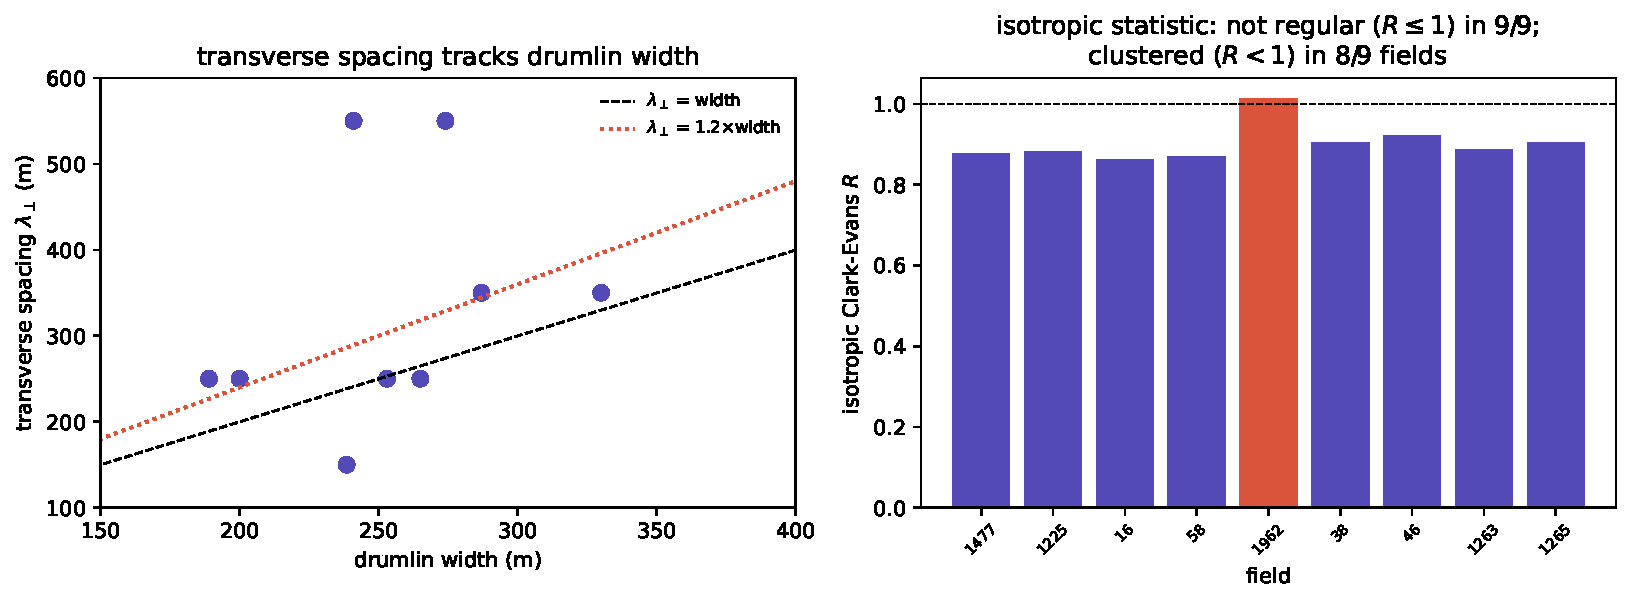
\includegraphics[width=\textwidth]{drumlin_summary.pdf}
\caption{(a) Transverse spacing $\lambda_\perp$ versus drumlin width across the nine fields;
$\lambda_\perp$ is of the same order as the width (dashed: equality; dotted: $1.2\times$). (b) Isotropic
Clark--Evans $R$ per field: $R\le1$ in all nine fields (clustered, $R<1$, in eight), confirming that
isotropic regularity is absent.}
\label{fig:summary}
\end{figure}

\section{Discussion}

\paragraph{An anisotropic, bedform-scale spacing.}
The single ``regular spacing'' attributed to drumlins resolves, on direction-resolved analysis, into two
opposite behaviours: along-flow \emph{clustering} (bedforms in trains) and across-flow
\emph{quasi-regularity} at a scale comparable to the drumlin width. The previously reported isotropic
regularity \citep{clark2018spatial} is consistent with this picture --- an isotropic statistic mixes a
clustered and a regular direction and returns an intermediate, weakly patterned signal --- but the
direction-resolved view localises the regularity to the transverse direction and ties its scale to the
bedform width.

\paragraph{Implications for instability theories.}
That the transverse spacing scales with the drumlin width is exactly what an instability theory predicts,
since a single wavelength sets both the size and the cross-flow spacing of the bedforms
\citep{hindmarsh1998,fowler2000,fowler2014,clark2009}. The same coincidence, however, means that
transverse spacing close to the width cannot by itself discriminate a pattern-forming instability from
simple steric packing of finite-width objects: at the first neighbour the two are observationally
degenerate, as the hard-rod comparison shows. Evidence for a genuine wavelength must come from the
\emph{longer-range} transverse order, which we find to be only weak. Spacing regularity alone is thus a
weak test of the instability hypothesis; size--spacing covariation and the persistence of transverse
order over several bedform widths are more diagnostic. This steric dominance of the mature pattern does
not in itself invalidate bed-instability models. A fluid-mechanical instability may still govern the
nucleation of bedforms and the early selection of a wavelength; but as a field matures, non-linear
saturation and the geometric crowding of finite-width bedforms can overprint that initial pattern, so
that the preserved record --- such as the BRITICE compilation of relict drumlins --- is effectively
truncated at the scale of the bedforms' own width. The instability hypothesis is therefore better tested
on active or immature fields, or through size--spacing covariation, than on mature spacing statistics.

\paragraph{Why anisotropic: shear flow versus buoyancy.}
The anisotropy itself is informative. Drumlins form within a continuous, directional basal shear flow,
which breaks the symmetry of the bed: sediment is advected and reworked along flow, favouring along-flow
continuity of bedforms (trains), much as in subaqueous and aeolian dunes, while the cross-flow direction
is free to take up a width-scale spacing. This differs from spacing systems driven by a vertical
buoyancy (Rayleigh--Taylor) instability with no imposed horizontal direction --- for example salt
structures, which can develop an isotropic, hard-core, liquid-like regular spacing in map view (without
reaching long-range, lattice-like order; \citealp{chen2026salt}). Whether an external flow direction is
imposed may thus be a first-order control on whether a geological spacing pattern is isotropically
regular or anisotropically clustered.

\paragraph{Not a hyperuniform pattern.}
Unlike some self-organised geological patterns, drumlin centroid fields show no suppression of
long-wavelength density fluctuations: the structure factor is patchiness-dominated at low wavenumber and
random at the spacing scale. The order in drumlin fields is local and transverse, not long-range.

\section{Conclusions}
\begin{itemize}\setlength\itemsep{1pt}
\item Resolved by direction, BRITICE drumlin spacing is strongly anisotropic: \emph{clustered} along ice
flow (bedforms in trains; isotropic Clark--Evans $R\le1$ in all nine fields) and \emph{quasi-regular}
across flow.
\item The transverse spacing $\lambda_\perp\!\approx\!250$\,m is of the same order as the drumlin width;
at the first neighbour it is largely accounted for by steric (non-overlap) packing, with only weak
longer-range transverse order beyond it.
\item The pattern is not hyperuniform; long-wavelength density fluctuations are not suppressed.
\item Isotropic spacing regularity is therefore a weak diagnostic of bed-instability theories for
drumlins; transverse, direction-resolved statistics and size--spacing covariation are required.
\end{itemize}

\section*{Data availability}
Drumlin outlines are from the BRITICE Glacial Map v2 \citep{clark2018britice}, freely available under a
Creative Commons Attribution licence from the University of Sheffield. All analysis code, the derived
drumlin-centroid table and the figure-generation scripts are openly available at
\url{https://github.com/Ruqing1963/drumlin-anisotropic-spacing}. Analysis used only open scientific
Python (NumPy, SciPy, Matplotlib).

\begin{thebibliography}{99}
\small
\bibitem[Baddeley et al.(2015)]{baddeley2015} Baddeley, A., Rubak, E., Turner, R., 2015.
\textit{Spatial Point Patterns: Methodology and Applications with R.} CRC Press.
\bibitem[Clark \& Evans(1954)]{clark1954} Clark, P.J., Evans, F.C., 1954. Distance to nearest neighbor as a
measure of spatial relationships in populations. \textit{Ecology} 35, 445--453.
\bibitem[Chen(2026)]{chen2026salt} Chen, R., 2026. Regular spacing of salt structures as a
Rayleigh--Taylor signature: edge-corrected point-pattern and structure-factor analysis of the U.S.\ Gulf
Coast and North German basins. Zenodo, doi:10.5281/zenodo.20834957.
\bibitem[Clark et al.(2009)]{clark2009} Clark, C.D., Hughes, A.L.C., Greenwood, S.L., Spagnolo, M., Ng,
F.S.L., 2009. Size and shape characteristics of drumlins, derived from a large sample, and associated
scaling laws. \textit{Quaternary Science Reviews} 28, 677--692.
\bibitem[Clark et al.(2018a)]{clark2018britice} Clark, C.D., Ely, J.C., Greenwood, S.L., Hughes, A.L.C.,
Meehan, R., Barr, I.D., Bateman, M.D., Bradwell, T., Doole, J., Evans, D.J.A., Jordan, C.J., Monteys, X.,
Pellicer, X.M., Sheehy, M., 2018. BRITICE Glacial Map, version 2: a map and GIS database of glacial
landforms of the last British--Irish Ice Sheet. \textit{Boreas} 47, 11--e8.
\bibitem[Clark et al.(2018b)]{clark2018spatial} Clark, C.D., Ely, J.C., Spagnolo, M., Hahn, U., Hughes,
A.L.C., Stokes, C.R., 2018. Spatial organization of drumlins. \textit{Earth Surface Processes and
Landforms} 43, 499--513.
\bibitem[Fowler(2000)]{fowler2000} Fowler, A.C., 2000. An instability mechanism for drumlin formation.
In: \textit{Deformation of Glacial Materials}, Geological Society Special Publication 176, 307--319.
\bibitem[Fowler \& Chapwanya(2014)]{fowler2014} Fowler, A.C., Chapwanya, M., 2014. An instability theory
for the formation of ribbed moraine, drumlins and mega-scale glacial lineations.
\textit{Proceedings of the Royal Society A} 470, 20140185.
\bibitem[Hindmarsh(1998)]{hindmarsh1998} Hindmarsh, R.C.A., 1998. The stability of a viscous till sheet
coupled with ice flow, considered at wavelengths less than the ice thickness. \textit{Journal of
Glaciology} 44, 285--292.
\bibitem[Ripley(1977)]{ripley1977} Ripley, B.D., 1977. Modelling spatial patterns. \textit{Journal of the
Royal Statistical Society B} 39, 172--212.
\bibitem[Torquato(2018)]{torquato2018} Torquato, S., 2018. Hyperuniform states of matter.
\textit{Physics Reports} 745, 1--95.
\end{thebibliography}

\end{document}
